\documentclass[apjl]{emulateapj}

\usepackage{hyperref}
\usepackage{amsmath}
\usepackage{amssymb}
\usepackage{graphicx}
\usepackage{color}
\usepackage{natbib}

\newcommand{\MSun}{M_\odot}
\newcommand{\RSun}{R_\odot}
\newcommand{\Rstar}{R_*}
\newcommand{\Mstar}{m_*}
\newcommand{\MBH}{M_\mathrm{BH}}

\def\aj{Astronomical Journal}                 % Astronomical Journal
\def\apj{Astrophysical Journal}                % Astrophysical Journal
\def\apjl{Astrophysical Journal}             % Astrophysical Journal, Letters
\def\pasj{PASJ}
\def\apjs{ApJS}              % Astrophysical Journal, Supplement
\def\mnras{MNRAS}            % Monthly Notices of the RAS
\def\prd{Phys.~Rev.~D}       % Physical Review D
\def\prl{Phys.~Rev.~Lett}    % Physical Review Letters
\def\cqg{Class.~Quant.~Grav.~}%Classical and Quantum Gravity
\def\araa{ARA\&A}             % Annual Review of Astron and Astrophys
\def\nat{Nature}              % Nature
\def\aap{A\&A}                % Astronomy and Astrophysics
\def\na{New Astronomy}

\newcommand{\will}[1]{\textcolor{cyan}{#1}}
\newcommand{\ilya}[1]{\textcolor{red}{#1}}

\newcommand{\onesigrange}[3]{\ensuremath{#1^{+#2}_{-#3}}}
\newcommand{\alpharange}{\onesigrange{2.27}{0.17}{0.15}}
\newcommand{\alpharangeHM}{\onesigrange{2.55}{0.23}{0.21}}

\begin{document}

\title{Comment on ``An excess of massive stars in the local 30 Doradus starburst''}

\author{Will Farr\altaffilmark{1}, Ilya Mandel\altaffilmark{1}}
\affil{$^1$Institute of Gravitational Wave Astronomy and School of Physics and Astronomy, University of Birmingham, Birmingham, B15 2TT, United Kingdom}
\email{wmfarr@star.sr.bham.ac.uk, imandel@star.sr.bham.ac.uk}

\begin{abstract}
Schneider et al.~(Reports, 5 January 2018, p.~69) found more massive stars in the 30 Doradus star-forming region above 30 solar masses than predicted by a standard Salpeter initial mass function (IMF).  Their finding of an IMF power-law exponent of $1.90^{+0.37}_{-0.26}$ is based on a flawed statistical analysis of the data.  We re-analyze their data with appropriate statistical tools to find an IMF exponent of $\alpharange$, consistent with the Salpeter value of $2.35$.
\end{abstract}

\maketitle

The universality of the initial mass function of stars is a hot topic in modern astrophysics, with impact on galactic evolution, supernovae, and gravitational-wave sources \cite{Kroupa:2002,Bastian:2010}.    \citet{Schneider:2018} use spectroscopic observations of young massive stars in the 30 Doradus region of the Large Magellanic Cloud to infer a shallower-than-expected IMF.  Their conclusion is due to a faulty statistical methodology.

\citet{Schneider:2018} obtain estimates of the ages and masses of individual stars with the BONNSAI Bayesian code \cite{Schneider:2017}.  They then obtain an overall mass distribution by effectively adding together the posterior probability density functions of individual stars.  There is no statistical meaning to a distribution obtained in this way, and it does not represent the posterior probability density function on the underlying mass distribution.  In fact, for a steeply decaying power law underlying distribution such as the one being considered here, the approach of \cite{Schneider:2018} will yield a distribution biased toward the high-mass end.  The measurement uncertainty will ``smear out'' the masses of both low-mass and high-mass stars, but because there are far more low-mass stars than high-mass ones, this appears to yield more mass at the high end of the distribution, leading to a false conclusion of a shallower distribution.

Hierarchical Bayesian inference provides the statistically correct solution to
this problem \cite{Hogg:2010}.  \citet{Mandel:2010stat} specifically considered
inference on a mass distribution given a sample of uncertain measurements, and
we use this methodology here.  We follow \citet{Schneider:2018} in assuming that
their data set is complete above 15 solar masses.  We interpret their inference
on individual masses and ages as independent Student T distributions for the log
of the mass and the age, with parameters fixed by matching the T location
parameter to the peak and the T scale parameter to the 68\% width of the
individual stellar distributions to the \citet{Schneider:2018} data.  We have
verified that the inference is robust to the number of degrees of freedom
assumed for the T distribution (see Figure \ref{fig:IMF}), suggesting that heavy
tails in the likelihood do not have a strong effect on the inference. We model
the star formation history as a truncated Gaussian distribution.  We impose
broad priors on the power-law slope and the mean and standard deviation of the
star formation Gaussian.    We use the Hamiltonian Monte Carlo sampler STAN
\citep{STAN} to efficiently address the high-dimensional hierarchical problem
with free parameters for each star's actual mass and birth age in addition to
the IMF slope and the mean and standard deviation of the star formation history.

Figure \ref{fig:IMF} shows the inferred power-law exponent of the IMF.  We find
an exponent of $\alpharange$ where the quoted value corresponds to the median of
the posterior distribution and the range to the 16th and 84th percentiles (i.e.\
the symmetric 68\% credible interval).  The conclusion is somewhat sensitive to
the choice of the cutoff mass for survey completeness, with an exponent of
$\alpharangeHM$ for a cutoff at $20 M_\odot$ rather than $15 M_\odot$ (not
shown).  However, these fluctuations are within the expected statistical
variation based on the sample size, as confirmed with posterior predictive
checking.  We see no reason to doubt the claim of \citet{Schneider:2018} that
the survey is complete for $M \geq 15 \, \MSun$.

\begin{figure}
%\vspace{-1in}
    		    		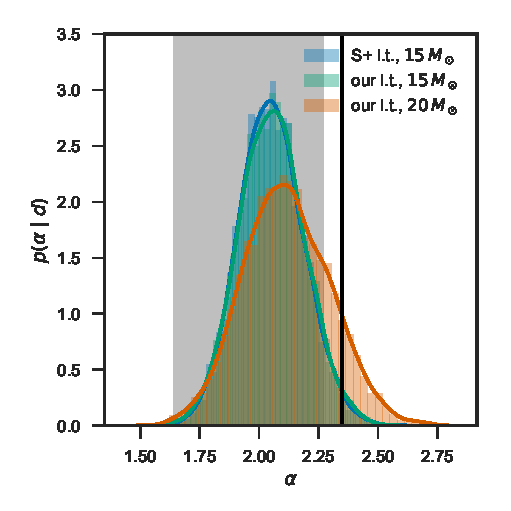
\includegraphics[width=\columnwidth]{alpha.pdf}
%\vspace{-1in}
    		\caption{The posterior inferred on the power law slope assuming survey completness for $M \geq 15 \, \MSun$ with $\nu = 100$ degrees of freedom in the Student T likelihood functions (blue curve; see text) and $\nu = 4$ degrees of freedom (green curve).  There is little difference between the blue and green curves, suggesting that the inference on the power law slope is insensitive to the heavy-tailed nature of the likelihood function.  In all cases the IMF slope we infer is consistent with a Salpeter slope of $-2.35$ \citep{Salpeter:1955}. }\label{fig:IMF}
\end{figure}

We confirm the stability of our conclusions with posterior predictive checking.
Figure \ref{fig:PPC} shows the distribution of observed masses and ages (i.e.\
the peak of the likelihood) from the \citet{Schneider:2018} data on top of the
range of mass and age distributions that would be observed from a large number
of data sets drawn according to our fitted IMF model.  The data can be seen to
be consistent with our IMF model.

\begin{figure}
%\vspace{-1in}
    		    		\includegraphics[width=\columnwidth]{dNdm-ppc-band.pdf}\\
                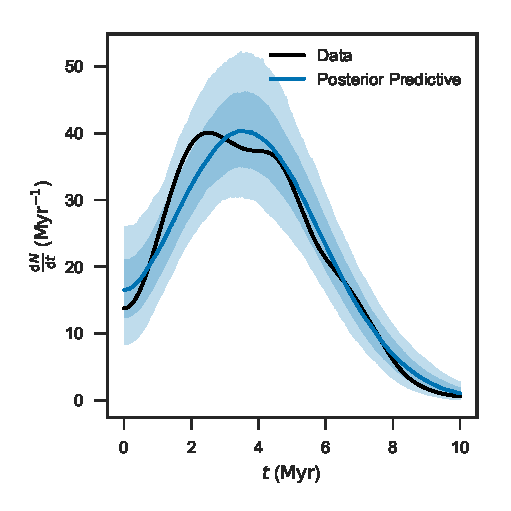
\includegraphics[width=\columnwidth]{dNdt-ppc-band.pdf}
%\vspace{-1in}
    		\caption{The observed distribution of (maximum likelihood) masses (top, black) and ages (bottom, black) and the range (median, 68\%, and 95\% credible intervals in blue) of distributions of mass and age from synthetic data drawn from our fitted model (i.e.\ the posterior predictive distribution).  We see no evidence that our model is unable to account for the features in the observed data, including the apparent shallowing of the slope of the mass distribution for $M \gtrsim 60 \, \MSun$.}\label{fig:PPC}
\end{figure}


In conclusion, we find that there is no evidence for a deviation from the Salpeter IMF in the observations of young massive stars in 30 Doradus once correct statistical analysis is applied.

\acknowledgments

While this note is critical of the conclusions in \citet{Schneider:2018}, those
authors should be commended for making the data on which their conclusions are
based available for further study and analysis.  This analysis made use of the \texttt{PySTAN} \citep{PySTAN}, \texttt{astropy} \citep{astropy}, \texttt{numpy} \citep{numpy}, \texttt{scipy} \citep{scipy}, \texttt{matplotlib} \citep{matplotlib}, and \texttt{seaborn} \citep{seaborn} Python libraries.

\bibliographystyle{hapj}
\bibliography{Mandel}
\end{document}
